\section{Results and Analysis}\label{sec:resultados}

\begin{table}[t]
\centering
\caption{Validation macro F1 by strategy (\%). The chosen one is in bold}
\label{tab:strategies}
\begin{tabular}{lrr}
\toprule
Strategy & ResNet-50 & MobileNetV3-L \\
\midrule
Head only & 84.8 & 89.4 \\
Last blocks, no augmentation & \textbf{93.5} & 93.2 \\
Last blocks, with augmentation & 92.4 & 94.4 \\
Full network, with augmentation & 93.0 & \textbf{94.5} \\
\bottomrule
\end{tabular}

\end{table}

\begin{figure*}[t]
\centering
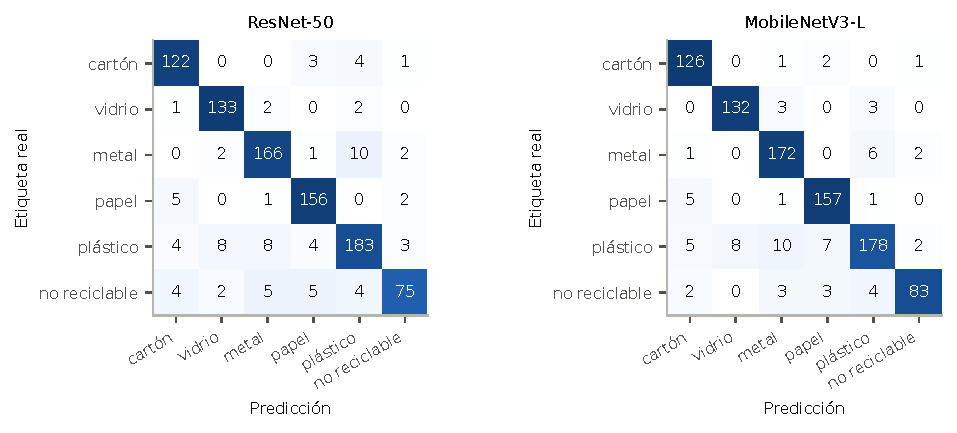
\includegraphics[width=0.66\textwidth]{confusion_matrices.pdf}
\caption{Test confusion matrices. Color indicates the proportion relative to the true class.}
\label{fig:confusion}
\end{figure*}

\begin{table*}[t]
\centering
\caption{Per-class test precision (P), recall (R), and F1 (\%)}
\label{tab:perclass}
\begin{tabular}{lrrrrrrr}
\toprule
Class & P (ResNet) & R (ResNet) & F1 (ResNet) & P (MobileNet) & R (MobileNet) & F1 (MobileNet) & $n$ \\
\midrule
cardboard & 89.7 & 93.8 & 91.7 & 90.6 & 96.9 & 93.7 & 130 \\
glass & 91.7 & 96.4 & 94.0 & 94.3 & 95.7 & 95.0 & 138 \\
metal & 91.2 & 91.7 & 91.5 & 90.5 & 95.0 & 92.7 & 181 \\
paper & 92.3 & 95.1 & 93.7 & 92.9 & 95.7 & 94.3 & 164 \\
plastic & 90.1 & 87.1 & 88.6 & 92.7 & 84.8 & 88.6 & 210 \\
non-recyclable & 90.4 & 78.9 & 84.3 & 94.3 & 87.4 & 90.7 & 95 \\
\bottomrule
\end{tabular}

\end{table*}

\subsection{Transfer Learning Strategies}

Table~\ref{tab:strategies} shows that freezing the entire extractor is the worst option for both networks. ImageNet features are not enough for materials distinguished by gloss, transparency, or texture, and fine-tuning the extractor improves macro F1 by 3.8 to 8.8 points. The three fine-tuning strategies are very close to one another. The effect of augmentation depends on the architecture: in MobileNet it improves the result, whereas in ResNet-50 partial fine-tuning without augmentation came out on top. That choice was kept because the criterion had been fixed in advance. As a consequence, the chosen ResNet is probably less tolerant of camera changes.

\begin{figure}[t]
\centering
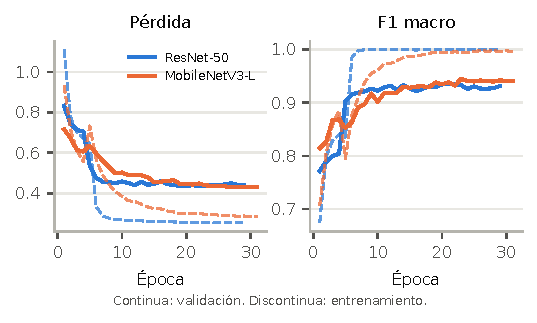
\includegraphics[width=\columnwidth]{vision_curves.pdf}
\caption{Curves of the chosen strategy for each architecture.}
\label{fig:vision-curves}
\end{figure}

In Fig.~\ref{fig:vision-curves}, the jump at epoch 5 marks the start of fine-tuning. The ResNet without augmentation reaches a training F1 of 1 within a few epochs, although its validation score remains stable. With augmentation, MobileNet's gap is smaller.

\begin{table}[t]
\centering
\caption{Classifiers on the test split}
\label{tab:vision}
\begin{tabular}{lrr}
\toprule
Métrica & ResNet-50 & MobileNetV3-L \\
\midrule
Accuracy (\%) & 91,0 & 92,4 \\
\quad IC 95\,\% & [89,0; 92,8] & [90,6; 94,0] \\
F1 macro (\%) & 90,6 & 92,5 \\
\quad IC 95\,\% & [88,5; 92,5] & [90,6; 94,1] \\
Precisión macro (\%) & 90,9 & 92,6 \\
Recall macro (\%) & 90,5 & 92,6 \\
Accuracy TrashNet (\%) & 92,9 & 93,4 \\
Accuracy RealWaste (\%) & 89,6 & 91,6 \\
Parámetros (millones) & 23,5 & 4,2 \\
Archivo, float16 (MB) & 47,2 & 8,6 \\
\bottomrule
\end{tabular}

\end{table}

\begin{figure*}[t]
\centering
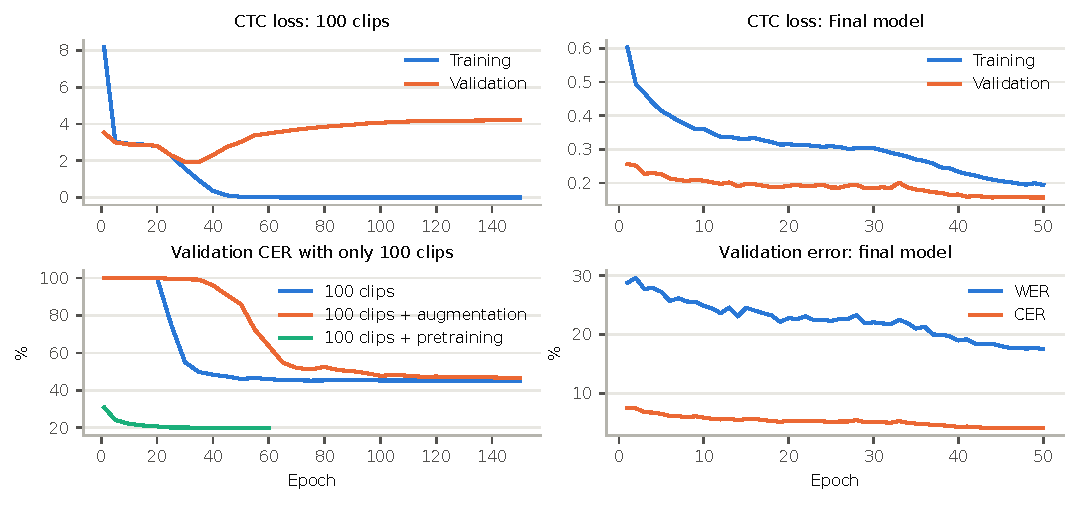
\includegraphics[width=0.74\textwidth]{speech_curves.pdf}
\caption{CTC training. Top: loss with 100 recordings and for the final model. Bottom: validation error.}
\label{fig:speech-curves}
\end{figure*}

\begin{table*}[t]
\centering
\caption{CTC experiments on the same validation set, with greedy decoding (\%). $N$: training recordings}
\label{tab:experiments}
\begin{tabular}{lrrrrr}
\toprule
Experiment & $N$ & WER unseen & CER unseen & WER TUX & CER TUX \\
\midrule
100 clips & 100 & 101.5 & 45.0 & 107.3 & 53.0 \\
100 clips + augmentation & 100 & 97.1 & 46.7 & 98.9 & 54.4 \\
TUX only (pretraining) & 10432 & 81.2 & 32.4 & 11.5 & 2.0 \\
100 clips + pretraining & 100 & 62.8 & 19.7 & 21.9 & 4.4 \\
Final model & 18779 & 29.9 & 7.8 & 10.9 & 2.0 \\
\bottomrule
\end{tabular}

\end{table*}

\subsection{Model Comparison on the Test Set}

MobileNetV3-Large achieved \MobAcc\,\% and ResNet-50 \ResAcc\,\% (Table~\ref{tab:vision}). Among the disagreements, only ResNet was correct on \McA{} images and only MobileNet on \McB{}. McNemar's test gives $p$ \McP, so \emph{neither network can be claimed to be more accurate than the other}. MobileNet was chosen for the application because of its better validation F1, its size, and its CPU latency. Both perform somewhat worse on RealWaste, where objects are dirty or deformed, but the gap with TrashNet is only a few points.

\begin{figure}[t]
\centering
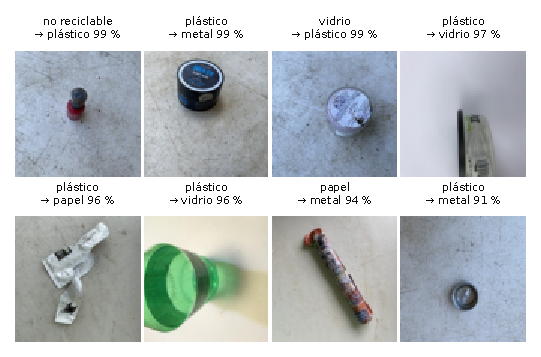
\includegraphics[width=0.78\columnwidth]{vision_errors.pdf}
\caption{Highest-confidence errors of MobileNetV3-L (true $\to$ predicted).}
\label{fig:errors}
\end{figure}

\begin{table*}[t]
\centering
\caption{Successes and failures on unseen speakers, taken from fixed positions of the WER ranking (\%)}
\label{tab:examples}
\small
\begin{tabular}{>{\raggedright\arraybackslash}p{0.44\textwidth}>{\raggedright\arraybackslash}p{0.44\textwidth}r}
\toprule
Reference & Transcription & WER \\
\midrule
ahora mismo en la isla de puerto rico hay cuarenta y cinco centros de acopio registrados & ahora mismo en la isla de puerto rico hay cuarenta y cinco centros de acopio registrados & 0 \\
me puedes mandar una foto de ella & me puedes mandar una foto de ella & 0 \\
me ayudas a plantar los naranjos & me ayudas a plantar los baranjos & 17 \\
el otro día ví un video en facebook sobre un aparatito que te ponías en la oreja y directamente te traducía & el otro día de un vida en frais por sobre en un aparatito que te ponía en la oreja y directamente de traducía & 33 \\
en el centro hay unos muy buenos bares con pantallas de plasma de sesenta pulgadas para disfrutar bien el partido & en el centro hay un es muy buenos varas con pantalla plaza de sesenta pulgas para es tu tar bien el partido & 50 \\
siempre he sido muy fan del color gris claro & siempresión muy tan el color desclaro & 78 \\
\bottomrule
\end{tabular}

\end{table*}

\subsection{Visual Error Analysis}
According to Table~\ref{tab:perclass} and Fig.~\ref{fig:confusion}, the hardest class for MobileNet is plastic, by recall: it is confused with metal (shiny surfaces), glass (transparency), paper (crumpled white packaging), and cardboard (printed containers). In ResNet, the trash (non-recyclable) class has the lowest recall. It is the smallest and most heterogeneous class, since it is defined by exclusion rather than by a material.

Fig.~\ref{fig:errors} shows the highest-confidence errors. Several are ambiguous even for a person: mixed-material containers, metal lids within the plastic class, or transparent green plastic that looks like glass. A confidence threshold does not eliminate these cases, but it does help. Calibration, with a temperature of \BestTemp{}, reduced the expected calibration error from \EceBefore\,\% to \EceAfter\,\%. With a threshold of 0.7, the model answers on \RejectCoverage\,\% of the test images and is correct on \RejectAcc\,\% of them.

\begin{table}[t]
\centering
\caption{Final model on validation and test (\%). $^{*}$\,$\alpha$ and $\beta$ were tuned on half of the validation set}
\label{tab:speech}
\resizebox{\columnwidth}{!}{\begin{tabular}{lrrrr}
\toprule
Decodificador & WER nuevos & CER nuevos & WER TUX & CER TUX \\
\midrule
Voraz & 35,1 & 9,7 & 10,8 & 1,9 \\
Beam & 35,1 & 9,6 & 10,5 & 1,8 \\
Beam + LM & 24,6 & 7,9 & 8,7 & 1,8 \\
\bottomrule
\end{tabular}
}
\end{table}

\begin{table}[t]
\centering
\caption{Test results by group, with beam search and language model (\%)}
\label{tab:speakers}
\begin{tabular}{lrrrr}
\toprule
Group & $n$ & WER & CER & Exact \\
\midrule
Unseen speakers & 278 & 24.6 & 7.9 & 17.6 \\
TUX speaker & 574 & 8.7 & 1.8 & 55.2 \\
Colombia, female & 60 & 28.0 & 9.7 & 16.7 \\
Colombia, male & 60 & 15.1 & 4.1 & 26.7 \\
Peru, female & 38 & 22.7 & 7.3 & 21.1 \\
Peru, male & 60 & 27.3 & 9.3 & 13.3 \\
Puerto Rico, female & 60 & 28.2 & 8.7 & 11.7 \\
\bottomrule
\end{tabular}

\end{table}

\subsection{Speech: What 100 Recordings Can Achieve}

From scratch, the 100 recordings lead to memorization: the training loss drops below 0.001 while the validation loss rises from its minimum (Fig.~\ref{fig:speech-curves}). The CER stalls at \ExpScratchCer\,\% and the WER at \ExpScratchWer\,\%, which exceeds 100\,\% because of insertions (Table~\ref{tab:experiments}). The curve also shows the initial phase typical of CTC: for about 20 epochs the network emits only blanks and the CER is 100\,\%.

\begin{figure}[t]
\centering
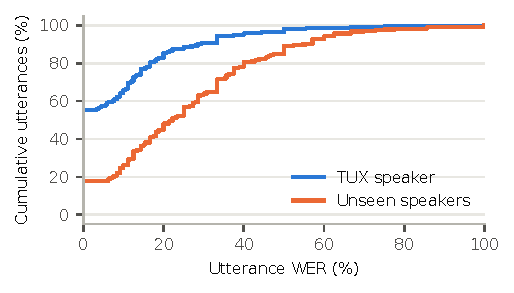
\includegraphics[width=0.70\columnwidth]{speech_distribution.pdf}
\caption{Cumulative distribution of per-utterance test WER.}
\label{fig:distribution}
\end{figure}

Data augmentation delays the exit from that phase and slows memorization, but it does \emph{not} improve the CER (\ExpAugCer\,\%). With so few examples, there is not enough variety of words and voices, and distorting the same recordings does not create it. Pretraining, in contrast, does change the outcome. The TUX model on its own fails on new voices (CER of \ExpTuxCer\,\%), but fine-tuning it on the same 100 recordings lowers the CER to \ExpTransferCer\,\%: the network already knows the mapping between Spanish sounds and letters and only needs to adapt to the voices. With the full corpus, it drops to \ExpMultiCer\,\%.

\begin{table}[t]
\centering
\caption{End-to-end latency on the demonstration machine}
\label{tab:latency}
\begin{tabular}{llr}
\toprule
Task & Hardware & Median / p95 \\
\midrule
Image, ResNet-50 & GPU & 6.1 / 8.8 ms \\
Image, MobileNetV3-L & GPU & 5.3 / 7.6 ms \\
Video 720p, ResNet-50 & GPU & 101.9 fps \\
Video 720p, MobileNetV3-L & GPU & 106.3 fps \\
5 s audio & GPU & 0.05 / 0.05 s \\
10 s audio & GPU & 0.09 / 0.10 s \\
Image, ResNet-50 & CPU & 30.2 / 32.7 ms \\
Image, MobileNetV3-L & CPU & 8.3 / 9.6 ms \\
Video 720p, ResNet-50 & CPU & 30.3 fps \\
Video 720p, MobileNetV3-L & CPU & 84.2 fps \\
5 s audio & CPU & 0.19 / 0.19 s \\
10 s audio & CPU & 0.38 / 0.39 s \\
\bottomrule
\end{tabular}

\end{table}

\subsection{Final Speech Model}

On validation, which was not used for training, the final model obtains a WER of \ValSlrWer\,\% and a CER of \ValSlrCer\,\% on unseen speakers (Table~\ref{tab:speech}). This figure is somewhat optimistic because alpha and beta were chosen on half of that set. On the test set, with unseen speakers and sentences, the WER is \SlrWer\,\% (95\,\% CI: \SlrWerLow{} to \SlrWerHigh) and the CER \SlrCer\,\%. Beam search without a language model barely changes the greedy output, because the network concentrates probability on a single path. Adding the language model lowers the WER from \SlrWerGreedy\,\% (Table~\ref{tab:speech}). The improvement is larger in WER than in CER: the n-gram corrects isolated letters and spaces that are enough to ruin a word.

With the TUX speaker, the WER is \TuxWer\,\%. The gap with respect to unseen speakers confirms that reporting only a sentence-level split would have given an overly optimistic picture. There are also marked differences between voices (Table~\ref{tab:speakers}), but each group has a single test speaker, so they reflect that person rather than a country or sex. Fig.~\ref{fig:distribution} shows the full error distribution.

In Table~\ref{tab:examples}, most failures are phonetically plausible. The most frequent character errors are missing or inserted spaces, a dropped \emph{s} (aspirated in parts of Latin American Spanish), the silent \emph{h}, confusions between \emph{b} and \emph{v}, which sound the same, and accent marks. The worst cases merge several words when speech is fast. Loanwords such as ``facebook'' fail because their spelling does not follow Spanish pronunciation.

\subsection{Video and Near Real Time}

Latency includes preprocessing, inference, and, depending on the case, video decoding, drawing, or beam search (Table~\ref{tab:latency}). All combinations exceed the thresholds of 5 frames per second and 5\,s per recording, even without a GPU. The 95th-percentile audio latency is \AudioLat\,s on GPU and \AudioLatCpu\,s on CPU. On GPU both networks are similar because preprocessing dominates. On CPU, MobileNet is more than three times faster per image. These figures do not include sending each frame to the browser.

The test video is our own montage of twelve test photos with simulated motion, rotation, and lighting changes, 62 frames per photo. MobileNet was correct on \VideoAcc\,\% of the frames. Failures concentrate on three photos that the model already misclassified as still images. Motion changed little: it corrected some frames of one of them and added some flicker, which smoothing reduces on screen. With twelve objects, this figure is a demonstration and not a performance estimate.

We also recorded two videos of our own with a phone (480$\times$864 pixels, 30 frames per second): a plastic water bottle (\OwnBottleFrames{} frames) and a notebook (\OwnNotebookFrames{} frames), on a white appliance, indoors under artificial light. Neither was used for training or tuning anything. MobileNetV3-L correctly classified \OwnBottleMob\,\% of the bottle frames and \OwnNotebookMob\,\% of the notebook frames; in the rest it confused the notebook with cardboard. ResNet-50 was correct on only \OwnBottleRes\,\% and \OwnNotebookRes\,\%: it saw glass in the transparent bottle and cardboard in the notebook. On the test set the two networks were indistinguishable, but with a real camera and outside both datasets the difference is huge. This is the clearest evidence in favor of data augmentation, which the chosen ResNet did not use, and of choosing MobileNet for the application. With two videos, it remains an observation and not a performance measurement.
